\documentclass[12pt]{article}
\usepackage{times} 			% use Times New Roman font

\usepackage[margin=1in]{geometry}   % sets 1 inch margins on all sides
\usepackage{hyperref}               % for URL formatting
\usepackage[pdftex]{graphicx}       % So includegraphics will work
\setlength{\parskip}{1em}           % skip 1em between paragraphs
\usepackage{indentfirst}            % indent the first line of each paragraph
\usepackage{datetime}
\usepackage[small, bf]{caption}
\usepackage{listings}               % for code listings
\usepackage{xcolor}                 % for styling code
\usepackage{multirow}

%New colors defined below
\definecolor{backcolour}{RGB}{246, 246, 246}   % 0xF6, 0xF6, 0xF6
\definecolor{codegreen}{RGB}{16, 124, 2}       % 0x10, 0x7C, 0x02
\definecolor{codepurple}{RGB}{170, 0, 217}     % 0xAA, 0x00, 0xD9
\definecolor{codered}{RGB}{154, 0, 18}         % 0x9A, 0x00, 0x12

%Code listing style named "gcolabstyle" - matches Google Colab
\lstdefinestyle{gcolabstyle}{
  basicstyle=\ttfamily\small,
  backgroundcolor=\color{backcolour},   
  commentstyle=\itshape\color{codegreen},
  keywordstyle=\color{codepurple},
  stringstyle=\color{codered},
  numberstyle=\ttfamily\footnotesize\color{darkgray}, 
  breakatwhitespace=false,         
  breaklines=true,                 
  captionpos=b,                    
  keepspaces=true,                 
  numbers=left,                    
  numbersep=5pt,                  
  showspaces=false,                
  showstringspaces=false,
  showtabs=false,                  
  tabsize=2
}

\lstset{style=gcolabstyle}      %set gcolabstyle code listing

% to make long URIs break nicely
\makeatletter
\g@addto@macro{\UrlBreaks}{\UrlOrds}
\makeatother

% for fancy page headings
\usepackage{fancyhdr}
\setlength{\headheight}{13.6pt} % to remove fancyhdr warning
\pagestyle{fancy}
\fancyhf{}
\rhead{\small \thepage}
\lhead{\small HW 8\, Venkatesh}  % EDIT THIS, REPLACE # with HW number
\chead{\small CS 532, Fall 2021} 

%-------------------------------------------------------------------------
\begin{document}

% EDIT THE ITEMS HERE
\begin{centering}
{\large\textbf{HW 8\ - Clustering}}\\ 
Swathi Venkatesh\\
12/05/2021\\
\end{centering}

%-------------------------------------------------------------------------

% The * after \section just says to not number the sections
\section*{Q1}
Generate a list of 100 popular accounts on Twitter. The accounts must be verified, have greater than 10,000 followers, and have greater than 5000 tweets. For example:

weiglemc - not verified, 509 followers, 2813 tweets - don't include
wnba - verified (blue checkmark), 739,600+ followers, 84,200+ tweets - could include
See Twarc API user\_lookup, GET users/lookup, and User object for details on obtaining this information for a set of accounts.

You may also generate this information manually by visiting individual account pages.

Because we're trying to cluster the accounts based on the text in their tweets, you should choose several sets of accounts that are similar (political, tech, sports, etc.) to see if they'll get clustered together later.

Save the list of accounts (screen\_names), one per line, in a text file named accounts.txt and upload to your GitHub repo.

\subsection*{Answer}

%Python code highlighting
\begin{lstlisting}[language=Python, caption=tweetparser.py , label=lst:copy]
#!/usr/local/bin/python3
from twarc import Twarc2, expansions
from configparser import ConfigParser

def userstat(twAuth,ids):
    #Find followers that are in this category and them to the list
    stat= False
    try:
        user = twAuth.get_user(id = ids)
        if user.verified and user.statuses_count >= 5000 and user.followers_count >= 10000 == True:
            stat = True
        else:
            stat = False
    except:
        print("Error")
    return stat

def setup_api(filename):
    '''
    filename: file where Twitter API keys are stored
    returns Twitter API object to pass into parse()
    '''

    # read Twitter API keys from twarc config file, setup twarc2 object
    config = ConfigParser(interpolation=None)
    with open(filename) as twarc_config:
        config.read_string("[TWARC]\n" + twarc_config.read())
    bearer_token = config['TWARC']['bearer_token'].strip('\'')
    t = Twarc2(bearer_token=bearer_token)
    return t

def parse(api, screen_name, num_tweets=100):
    '''
    api: Twitter API object, use setup_api() to create
    screen_name: Twitter screen_name
    num_tweets: Number of tweets to request (default: 100)
    returns dict with {'screen_name': screen_name, 'tweets': [tweet1, tweet2, ...]}
    '''

    tweet_data = []
    try:
        timeline = api.timeline(screen_name, max_results=num_tweets, exclude_replies=True, exclude_retweets=True)
        for page in timeline:
            result = expansions.flatten(page)
            for tweet in result:
               tweet_data.append(tweet["text"])
               if len(tweet_data) == num_tweets:
                    # must include this to stop after a certain # of tweets
                    timeline.close()
    except Exception as e:
        print ("Twarc Error: %s" % str(e))
  
    account_data = {'screen_name': screen_name, 'tweets': tweet_data}
    return account_data

\end{lstlisting}

%Python code highlighting
\begin{lstlisting}[language=Python, caption=twittergatherid.py , label=lst:copy]
#!/usr/local/bin/python3
from twarc import Twarc2, expansions
from tweetparser import setup_api, user_stat
import pandas as pd
import numpy as np
def  twitter_account(types,api= setup_api("/config") ):
    
    #Get twitter friends screen_name of the parse account, as one arrayList
    public_tweets = twarc.user_lookup(api.friends_ids, id = types)
    count= 1
    resultList =[] # store the final result of screen names
    for user in public_tweets.pages():
        #print(user)
        #print(user.dtypes())
        #Transverse the list of followers ids
        for i in user:
            #check if requirement is met
            if(user_stat(api,i) ==True):
                if( i not in resultList):   
                    #instead of the user id get the user name
                    user_sc = api.get_user(i)
                    print("{}:{}".format(count,user_sc.screen_name))
                    resultList.append(user_sc.screen_name)
                    count += 1                    
            #Get maximum 30 file accounts screen_names
            if(count >= 30):
                break
    print(resultList)

    #build text file and save file in q1 directory
    filename =  'one/' + types + '.txt'
    with open(filename, 'w') as filehandle:
        for listitem in resultList:
            filehandle.write('%s\n' % listitem)
    return resultList
"""
Tech= @WIRED
Sport= @WNBA
politics = @POTUS45
music = @future_of_music



"""
#Get all screen_names with that fulfils 10,000 followers and have 5000 tweets and verified
twitter_account("WIRED")
twitter_account("WNBA")
twitter_account("POTUS45")
twitter_account("future_of_music")


"""
Bring all result from the files in to One text file 
accounts.txt
"""
#get the list of the created files
column_name= ["User_screen_names"]
final = pd.DataFrame(columns= column_name)
fileList = ["one/WIRED.txt","one/WNBA.txt","one/POTUS45.txt","one/future_of_music.txt"]
df = pd.DataFrame()


for t in fileList:
    frame = pd.read_csv(t,header=None)
    frame.columns = column_name
    for ind in frame.index:
        final.loc[len(final)] =[frame['User_screen_names'][ind]]
        

# dropping duplicate values
final.User_screen_names.drop_duplicates(inplace=True)  

#confirm that there are all unique values 
print(final.User_screen_names.nunique())

# Number of rows to drop
n = 14
  
# Dropping last n rows using drop
final.drop(final.tail(n).index,
        inplace = True)
#print(final.User_screen_names.nunique())
numpy_array = final.to_numpy()
#print as a text file 
np.savetxt(r'accounts.txt', numpy_array,fmt="%s")


\end{lstlisting}

\subsection*{Discussion}

The following consideration is made for gathering the user screen names. The screen names were collected through popular twitter accounts WNBA, POTUS45, future of music and WIRED. The lines 5-16 handles account that check screen\_name account meets requirements.
\lstinputlisting[language=Python,caption=A snap shot of tweetparser.py, label=twitter1:import,firstnumber=5,firstline=5,lastline=16]{tweetparser.py} 

\emph{Q: How did you choose to collect the accounts?}

Function twitter\_account() produce a text files (names based on the arguement supplied) that gets stored in /one folder.

\lstinputlisting[language=Python,caption=A snap shot of twittergatherid.py, label=twitter2:import,firstnumber=52,firstline=52,lastline=85]{twittergatherid.py} 

\emph{Q: What topics/categories do the accounts belong to? You don't need to specify a grouping for each account, but what general topics/categories will you expect to be revealed by the clustering?}

The topics belong to technology, sports, politics and music categories.

\section*{Q2}

\subsection*{Answer}

%Python code highlighting
\begin{lstlisting}[language=Python, caption=generatetweetvector.py , label=2nd:copy]
#!/usr/local/bin/python3
from tweetparser import setup_api, parse
import re

def getwordcounts(api, screen_name):
    """
    api: Twitter API object
    screen_name: Twitter screen_name
    returns screen_name and dictionary of word counts for a Twitter account
    """
    
    # Parse the Twitter feed
    d = parse(api, screen_name)
    wc = {}

    # Loop over all the entries
    for tweet in d['tweets']:

        # Extract a list of words
        words = getwords(tweet)
        for word in words:
            wc.setdefault(word, 0)
            wc[word] += 1

    return (d['screen_name'], wc)

def getwords(tweet):
    """
    returns lowercase list of words after filtering
    """

    # Remove URLs
    text = re.compile(r'(http://|https://|www\.)([^ \'\"]*)').sub('', tweet)
    "
    # Remove other screen names (start with @)
    text = re.compile(r'(@\w+)').sub('', text)

    # Split words by all non-alpha characters
    words = re.compile(r'[^A-Z^a-z]+').split(text)

    # Filter for words between 3-15 characters, convert to lowercase, and return as a list
    return [word.lower() for word in words if (len(word) >= 3 and len(word) <= 15)]

#####
# MAIN CODE STARTS HERE
#####


# set up Twitter API object
api = setup_api("/config")

apcount = {}      # number of accounts each word appears in
wordcounts = {}   # words and frequency in each account
sumcounts = {}    # words and frequency over all accounts (to determine most popular)

# list of screen names should be in 'accounts.txt', one per line
accountlist = [line.strip() for line in open('accounts.txt')]
#print(accountlist)
#print(len(accountlist))

for screen_name in accountlist:
    try:
        # get tweets, filter and count words
        (user, wc) = getwordcounts(api, screen_name)
        wordcounts[user] = wc
        
        # count number of accounts each term appears in
        for (word, count) in wc.items():
            apcount.setdefault(word, 0)
            sumcounts.setdefault(word, 0)
            if count > 1:
                apcount[word] += 1        # counting accounts with the word
                sumcounts[word] += count  # summing total counts for the word
    except:
        print ('Failed to parse account %s' % screen_name)
        

#print("Counting words done")
#print(sumcounts.keys())

# remove stopwords ("fake" way)
wordlist = []
for (w, ac) in apcount.items():
    # w is the word, ac is the account count (was bc 'blog count' in textbook)
    frac = float(ac) / len(accountlist)
    if frac > 0.1 and frac < 0.5:
        wordlist.append(w)

popularlist = []

#### 
# BEGIN YOUR CODE BLOCK
####

#tuple list sorted by index 1 i.e. value field
l = sorted(sumcounts.items() , key=lambda x: x[1],reverse=True)
#extract 500 rows 
l = l[:500]
#store in the dictionary
popularlist = [i[0] for i in l]

# write out popular word list
with open('popularlist.txt', 'w') as outf:
    for word in popularlist:
        outf.write(word + '\n')

# write out account-term matrix
with open('tweetdata.txt', 'w') as outf:
    # write header row ("Account", list of words)
    outf.write('Account')
    for word in popularlist:
        outf.write('\t%s' % word)
    outf.write('\n')

    # write each row (screen_name, count for each word)
    for (screen_name, wc) in wordcounts.items():
        outf.write(screen_name)
        for word in popularlist:
            if word in wc:
                outf.write('\t%d' % wc[word])
            else:
                outf.write('\t0')
        outf.write('\n')


\end{lstlisting}

\subsection*{Discussion}

\begin{itemize}
\item \emph{Q:Explain the general operation of generatetweetvector.py and how the tweets are converted to the account-term matrix.}

\item The code drive started from line 56 to line 123.

\item From lines 61 to 75, uses a major function called getwordcounts(api,screen name). In this function the parse(api,screen name) is called. The parse function returns users tweets full text that are not retweets nor replies. When that full tweet text is gotten for a particular user, getwords(tweet) function removes unwanted text from the tweets gotten such as URLS and Mentions. It then extracts word that has at least 3 to 15 length size in each sentence in the tweets and converts them to lower cases.

\item The result is stored for each words in a dictionary where by if the word repeats itself again the word(which is the key of the dictionary) increments the values by one.

\item getwordcounts returns the screen name with a dictionary or words with its frequency count as well.

\item Moving we count the number of accounts each term appear. It is noticed that each works and users account are stored in a variable outside the for loop; so basically result gotten gets added on each screen names.

\item It appears to keep track of the overall frequency of the word too for every user combined.

\item Then the removal of stop words (this is calculated, not gotten from a list of unwanted words) is done. It basically gets the word count divided by the total number of account names gotten from the accounts.txt, once it satisfies a particular fraction between 0.1 and 0.5 the word is added to the group of wordlist.

\item \emph{Q: Explain in detail the code that you added to filter for the 500 most frequent non-stopword terms.}

\item For the popular list the items were sorted using the lambda function and the results were placed in the variable l. This variable l is a list of tuple. It goes from highest to lowest. Only 500 row items were considered by splicing the tuple and they were stored in a dictionary variable called popularlist.

\item Finally, results of popularlist variable words are saved in a text file while tweetdata.txt as a header of the popularlist or words and the screen name with count of each word on a single row.

\item \emph{Q: Do the 500 most frequent terms make sense based on the accounts that you chose?}

\item The word i viewed in popularlist.txt makes a lot of sense because it is as a form of connection to sports, politics, music or tech considered.


\end{itemize}

\section*{Q3}

\subsection*{Answer}

%Python code highlighting
\begin{lstlisting}[language=Python, caption=three.py , label=2nd:copy]
#!/usr/local/bin/python3
from PIL import Image, ImageDraw
from math import sqrt
import random
import csv
import pandas as pd
def readfile(filename):
  data = []
  rownames = []
  colnames = []
  num_rows = 0
  with open(filename) as tsvfile:
    reader = csv.reader(tsvfile, delimiter='\t')
    for row in reader:
      if num_rows > 0:
        rownames.append(row[0])    # save the row names
        data.append([float(x) for x in row[1:]])  # save the values as floats
      else:
        for col in row[1:]:
          colnames.append(col)    # save the column names
      num_rows = num_rows + 1
  return (rownames, colnames, data)

def pearson(v1, v2):
  # Simple sums
    sum1 = sum(v1)
    sum2 = sum(v2)

  # Sums of the squares
    sum1Sq = sum([pow(v, 2) for v in v1])
    sum2Sq = sum([pow(v, 2) for v in v2])

  # Sum of the products
    pSum = sum([v1[i] * v2[i] for i in range(len(v1))])

  # Calculate r (Pearson score)
    num = pSum - sum1 * sum2 / len(v1)
    den = sqrt((sum1Sq - pow(sum1, 2) / len(v1)) * (sum2Sq - pow(sum2, 2)
               / len(v1)))
    if den == 0:
        return 0

    return 1.0 - num / den        
"""
MD5 Scaling
"""
def scaledown(data, distance=pearson, rate=0.01):
    n = len(data)

  # The real distances between every pair of items
    realdist = [[distance(data[i], data[j]) for j in range(n)] for i in
                range(0, n)]

  # Randomly initialize the starting points of the locations in 2D
    loc = [[random.random(), random.random()] for i in range(n)]
    fakedist = [[0.0 for j in range(n)] for i in range(n)]

    lasterror = None
    for m in range(0, 1000):
    # Find projected distances
        for i in range(n):
            for j in range(n):
                fakedist[i][j] = sqrt(sum([pow(loc[i][x] - loc[j][x], 2)
                                      for x in range(len(loc[i]))]))

    # Move points
        grad = [[0.0, 0.0] for i in range(n)]

        totalerror = 0
        for k in range(n):
            for j in range(n):
                if j == k:
                    continue
        # The error is percent difference between the distances
                errorterm = (fakedist[j][k] - realdist[j][k]) / realdist[j][k]

        # Each point needs to be moved away from or towards the other
        # point in proportion to how much error it has
                grad[k][0] += (loc[k][0] - loc[j][0]) / fakedist[j][k] \
                    * errorterm
                grad[k][1] += (loc[k][1] - loc[j][1]) / fakedist[j][k] \
                    * errorterm

        # Keep track of the total error
                totalerror += abs(errorterm)
        print (totalerror)

    # If the answer got worse by moving the points, we are done
        if lasterror and lasterror < totalerror:
            break
        lasterror = totalerror

    # Move each of the points by the learning rate times the gradient
        for k in range(n):
            loc[k][0] -= rate * grad[k][0]
            loc[k][1] -= rate * grad[k][1]

    return loc

def draw2d(data, labels, jpeg):
    img = Image.new('RGB', (2000, 2000), (255, 255, 255))
    draw = ImageDraw.Draw(img)
    for i in range(len(data)):
        x = (data[i][0] + 0.5) * 1000
        y = (data[i][1] + 0.5) * 1000
        draw.text((x, y), labels[i], (0, 0, 0))
    img.save(jpeg, 'JPEG')

def rotatematrix(data):
    newdata = []
    for i in range(len(data[0])):
        newrow = [data[j][i] for j in range(len(data))]
        newdata.append(newrow)
    return newdata

"""
Hierarchical Clustering
class bicluster - data structure to hold the clustering information
hcluster(rows, distance=pearson) - does the hierarchical clustering, default distance function is pearson()
printclust(clust, labels=None, n=0) - traverses the cluster and prints an ASCII text representation
"""      
class bicluster:

    def __init__(self, vec, left=None, right=None, distance=0.0, id=None,):
        self.left = left
        self.right = right
        self.vec = vec
        self.id = id
        self.distance = distance

def hcluster(rows, distance=pearson):
    distances = {}
    currentclustid = -1

  # Clusters are initially just the rows
    clust = [bicluster(rows[i], id=i) for i in range(len(rows))]

    while len(clust) > 1:
        lowestpair = (0, 1)
        closest = distance(clust[0].vec, clust[1].vec)

    # loop through every pair looking for the smallest distance
        for i in range(len(clust)):
            for j in range(i + 1, len(clust)):
        # distances is the cache of distance calculations
                if (clust[i].id, clust[j].id) not in distances:
                    distances[(clust[i].id, clust[j].id)] = \
                        distance(clust[i].vec, clust[j].vec)

                d = distances[(clust[i].id, clust[j].id)]

                if d < closest:
                    closest = d
                    lowestpair = (i, j)

    # calculate the average of the two clusters
        mergevec = [(clust[lowestpair[0]].vec[i] + clust[lowestpair[1]].vec[i])
                    / 2.0 for i in range(len(clust[0].vec))]

    # create the new cluster
        newcluster = bicluster(mergevec, left=clust[lowestpair[0]],
                               right=clust[lowestpair[1]], distance=closest,
                               id=currentclustid)

    # cluster ids that weren't in the original set are negative
        currentclustid -= 1
        del clust[lowestpair[1]]
        del clust[lowestpair[0]]
        clust.append(newcluster)

    return clust[0]


def printclust(clust, labels=None, n=0):
  # indent to make a hierarchy layout
    for i in range(n):
        print (' ', end =" ")
    if clust.id < 0:
    # negative id means that this is branch
        print ('-')
    else:
    # positive id means that this is an endpoint
        if labels == None:
            print (clust.id)
        else:
            print (labels[clust.id])

  # now print the right and left branches
    if clust.left != None:
        printclust(clust.left, labels=labels, n=n + 1)
    if clust.right != None:
        printclust(clust.right, labels=labels, n=n + 1)

"""
Dendrogram
"""
def getheight(clust):
  # Is this an endpoint? Then the height is just 1
    if clust.left == None and clust.right == None:
        return 1

  # Otherwise the height is the same of the heights of
  # each branch
    return getheight(clust.left) + getheight(clust.right)


def getdepth(clust):
  # The distance of an endpoint is 0.0
    if clust.left == None and clust.right == None:
        return 0

  # The distance of a branch is the greater of its two sides
  # plus its own distance
    return max(getdepth(clust.left), getdepth(clust.right)) + clust.distance

def drawdendrogram(clust, labels, jpeg='clusters.jpg'):
  # height and width
    h = getheight(clust) * 20
    w = 1200
    depth = getdepth(clust)

  # width is fixed, so scale distances accordingly
    scaling = float(w - 150) / depth

  # Create a new image with a white background
    img = Image.new('RGB', (w, h), (255, 255, 255))
    draw = ImageDraw.Draw(img)

    draw.line((0, h / 2, 10, h / 2), fill=(255, 0, 0))

  # Draw the first node
    drawnode(
        draw,
        clust,
        10,
        h / 2,
        scaling,
        labels,
        )
    img.save(jpeg, 'JPEG')
    
def drawnode(
    draw,
    clust,
    x,
    y,
    scaling,
    labels,
    ):
    if clust.id < 0:
        h1 = getheight(clust.left) * 20
        h2 = getheight(clust.right) * 20
        top = y - (h1 + h2) / 2
        bottom = y + (h1 + h2) / 2
    # Line length
        ll = clust.distance * scaling
    # Vertical line from this cluster to children
        draw.line((x, top + h1 / 2, x, bottom - h2 / 2), fill=(255, 0, 0))

    # Horizontal line to left item
        draw.line((x, top + h1 / 2, x + ll, top + h1 / 2), fill=(255, 0, 0))

    # Horizontal line to right item
        draw.line((x, bottom - h2 / 2, x + ll, bottom - h2 / 2), fill=(255, 0,
                  0))

    # Call the function to draw the left and right nodes
        drawnode(
            draw,
            clust.left,
            x + ll,
            top + h1 / 2,
            scaling,
            labels,
            )
        drawnode(
            draw,
            clust.right,
            x + ll,
            bottom - h2 / 2,
            scaling,
            labels,
            )
    else:
    # If this is an endpoint, draw the item label
        draw.text((x + 5, y - 7), labels[clust.id], (0, 0, 0))
"""
K-Means Clustering
"""       
def kcluster(rows,k,distance=pearson ):
  # Determine the minimum and maximum values for each point
    ranges = [(min([row[i] for row in rows]), max([row[i] for row in rows]))
              for i in range(len(rows[0]))]

  # Create k randomly placed centroids
    clusters = [[random.random() * (ranges[i][1] - ranges[i][0]) + ranges[i][0]
                for i in range(len(rows[0]))] for j in range(k)]

    lastmatches = None
    for t in range(100):
        print ('Iteration %d' % t)
        bestmatches = [[] for i in range(k)]

    # Find which centroid is the closest for each row
        for j in range(len(rows)):
            row = rows[j]
            bestmatch = 0
            for i in range(k):
                d = distance(clusters[i], row)
                if d < distance(clusters[bestmatch], row):
                    bestmatch = i
            bestmatches[bestmatch].append(j)

    # If the results are the same as last time, this is complete
        if bestmatches == lastmatches:
            break
        lastmatches = bestmatches

    # Move the centroids to the average of their members
        for i in range(k):
            avgs = [0.0] * len(rows[0])
            if len(bestmatches[i]) > 0:
                for rowid in bestmatches[i]:
                    for m in range(len(rows[rowid])):
                        avgs[m] += rows[rowid][m]
                for j in range(len(avgs)):
                    avgs[j] /= len(bestmatches[i])
                clusters[i] = avgs

    return bestmatches

"""
Q3 
"""
tweetdata, word,data =readfile("tweetdata.txt")
clust = hcluster(data)
#print(clust.vec)

"""
Q3  ASCIII
To view  cluster
"""
printclust(clust,labels=tweetdata)


"""
Q3 Dendrogram
"""
drawdendrogram(clust,tweetdata,jpeg="three/tweetdata.jpeg")

"""
Q4
"""
"""
For 5  kcluster
number of iteration:
    Iteration 0
    Iteration 1
    Iteration 2
    Iteration 3
    Iteration 4
    Iteration 5
    Iteration 6
    Iteration 7
    Iteration 8
    Iteration 9
    Iteration 10
    Iteration 11
    Iteration 12
Cluster summary:
    cluster  1 :  1
    cluster  2 :  39
    cluster  3 :  36
    cluster  4 :  20
    cluster  5 :  2
"""


clust5 = kcluster(data,5)
for i in range(len(clust5)):
  print ("cluster ", i+1, ": ", len(clust5[i]))
  for r in clust5[i]:
      f= 'four/clust5cluster'+ str(i+1)+'.csv'
      with open(f, 'a+') as file:
          file.write(tweetdata[r])
          file.write("\n")

"""
For 10  kcluster
number of iteration:
    Iteration 0
    Iteration 1
    Iteration 2
    Iteration 3
Cluster summary:   
    cluster  1 :  0
    cluster  2 :  0
    cluster  3 :  88
    cluster  4 :  4
    cluster  5 :  0
    cluster  6 :  0
    cluster  7 :  6
    cluster  8 :  0
    cluster  9 :  0
    cluster  10 :  0
"""


clust10 = kcluster(data,10)
for i in range(len(clust10)):
  print ("cluster ", i+1, ": ", len(clust10[i]))
  for r in clust10[i]:    
      f= 'four/clust10cluster'+ str(i+1)+'.csv'
      with open(f, 'a+') as file:
          file.write(tweetdata[r])
          file.write("\n")

"""
For 20  kcluster
number of iteration:
    Iteration 0
    Iteration 1
    Iteration 2
    Iteration 3
    Iteration 4
    Iteration 5
    Iteration 6
    Iteration 7
    Iteration 8
    Iteration 9
    Iteration 10
    Iteration 11
    Iteration 12
    Iteration 13
    Iteration 14
clusters summary:
    cluster  1 :  1
    cluster  2 :  1
    cluster  3 :  0
    cluster  4 :  0
    cluster  5 :  0
    cluster  6 :  0
    cluster  7 :  0
    cluster  8 :  0
    cluster  9 :  39
    cluster  10 :  2
    cluster  11 :  0
    cluster  12 :  0
    cluster  13 :  6
    cluster  14 :  0
    cluster  15 :  0
    cluster  16 :  5
    cluster  17 :  0
    cluster  18 :  0
    cluster  19 :  44
    cluster  20 :  0
"""


clust20 = kcluster(data,20)
for i in range(len(clust20)):
  print ("cluster ", i+1, ": ", len(clust20[i]))
  f= 'four/clust20cluster'+ str(i+1)+'.csv'
  for r in clust20[i]:
      with open(f, 'a+') as file:
          file.write(tweetdata[r])
          file.write("\n")

"""
Q5='mds2d.jpg'
25602.68055067695
175394.90708243262
98
"""


coords = scaledown(data)
print(len(coords))
draw2d(coords, tweetdata, jpeg='five/mds2d.jpg')

\end{lstlisting}


\subsection*{Discussion}
In getting the ASCII and Dendrogram the following had to be put in place:

\begin{itemize}
\item Line 339 to 350 is the drive for the code.

\lstinputlisting[language=Python,caption= Driver code for Q3, label=three:import,firstnumber=339,firstline=339,lastline=350]{three.py}

\item Used the readfile() function to read in the text, it gets all data and returns the user-names as row names, the words as col names, and the value as data(data stored as a 2D array
of float values).

\item  Then the data is passed in hcluster(data) also known as  hierarchical clustering, this function used the pearson() function when called.

\item The pearson function takes two vector arrays as arguments and then returns the pearson correlation between these values.

\item hcluster() function also uses a bi-cluster class which is an helper for comparing two clusters.

\item hcluster does the hierarchical clustering by agglomerative clustering which involves merging the best matches cluster with a new cluster. It repeats this cycle untill there is just one cluster left.

\item printclust() function prints recursively the final end product of the hclusters returned function.The printcluster has an argument called labels, the label when removed prints the cluster based on the position number of accounts names but when the label is supplied it prints the actual name of the labels. Print produces the ASCII text of the output. It is saved in as ascii.txt in /three.

\item drawdendrogram() does the similar objective as the printcluster but it produces a jpeg format of the recursive output of the cluster.

\end{itemize}

\clearpage
\begin{figure}[h]
\centering
% trim and clip are used to crop the image, trim=left bottom right top
% width sets max width, height will be scaled appropriately
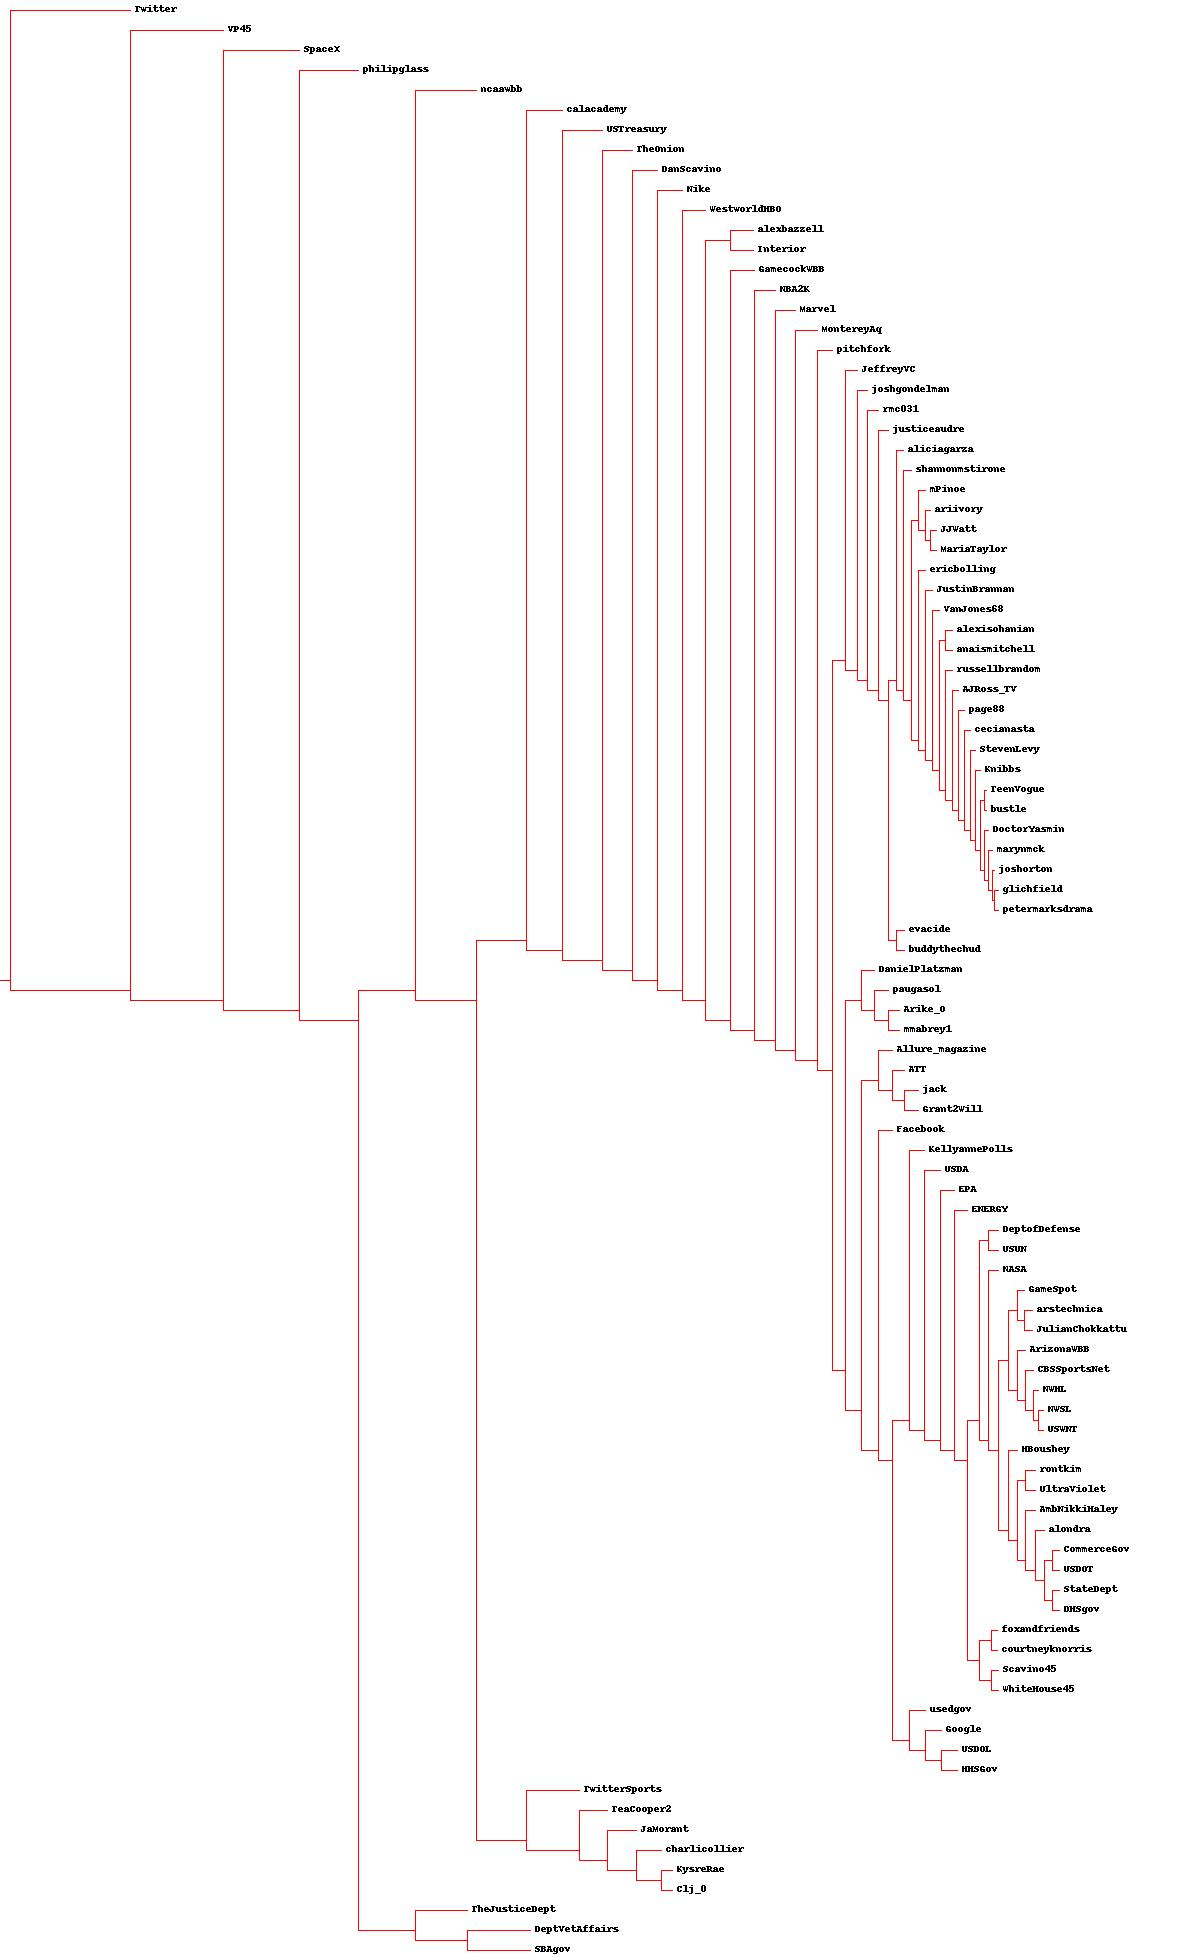
\includegraphics[width=\textwidth,height=\textheight,keepaspectratio]{tweetdata.jpeg}
\caption{ Question 3 output}
\label{fig}
\end{figure}
\clearpage
\section*{Q4}

\subsection*{Answer}

\lstinputlisting[language=Python,caption= Driver code for Q4 , label=Q4:import,firstnumber=351,firstline=351,lastline=467]{three.py}

\subsection*{Discussion}

\begin{itemize}
\item Q: Give a brief explanation of how the k-Means algorithm operates on this data. What features is the algorithm considering?

Q: How many iterations were required for each value of k?

Q: Which k value created the most reasonable clusters? For that grouping, characterize the accounts that were clustered into each group.

\item K-mean algorithm work in the manner.

\item in the kcluster function, it first try to organize the data in ranges of minimum and maximum values for each row so that the clusters can be represents as a coordinate in 2d form.

\item The last part is update the clusters average(mean) to their new members, this changes the location of the clusters and groups them together and closer based on the average of all the group members.

\item Final check is to make sure that the best is the matches is the list of rows in each clusters. This ensure the group members are more close together on average.

\item kcluster = 5 had 12 iteration starting from zero and produced a total of 5 clusters. 

\lstinputlisting[language=Python,caption= kcluster 5 , label=Q4:import,firstnumber=354,firstline=354,lastline=376]{three.py}

\item kcluster = 10 had 3 iteration starting from zero and produced a total of 10 clusters. 

\lstinputlisting[language=Python,caption= kcluster 10 , label=Q4:import,firstnumber=388,firstline=388,lastline=406]{three.py}

\item kcluster = 20 had 14 iteration starting from zero and produced a total of 20 clusters. 

\lstinputlisting[language=Python,caption= kcluster 20 , label=Q4:import,firstnumber=418,firstline=418,lastline=457]{three.py}

\item From all the list of clusters made I would say none of them satisfied a uniform grouping but if I would have to choose k equals 10 is better.

\item The code for each k values of 5,10 and 20 writes the twitter screen names row by row for each cluster based on the cluster summary. Each cluster gets a particular file name.

\lstinputlisting[language=Python,caption= kcluster 20 , label=Q4:import,firstnumber=379,firstline=379,lastline=386]{three.py}

\end{itemize}

\section*{Q5}

\subsection*{Answer}
The mds2d.jpg is added in the next page.
\begin{figure}[h]
\centering
% trim and clip are used to crop the image, trim=left bottom right top
% width sets max width, height will be scaled appropriately

\includegraphics[width=\textwidth,height=\textheight,keepaspectratio]{mds2d.jpg}
\caption{ Question 5 output}
\label{fig}
\end{figure}

\subsection*{Discussion}
\begin{itemize}
\item Q: How many iterations were required?

Q: How well did the MDS do in grouping similar accounts together? Were there any particularly odd groupings?

\item This is the resulting output.

\item There were 98 iteration in total by checking the length of coord in line 478.

\lstinputlisting[language=Python,caption= Driver for Q5 , label=Q5:import,firstnumber=477,firstline=477,lastline=479]{three.py}

\item MDS did fairly good in grouping similar accounts together. Considering philipglass and SBAgov which is grouped together, actually is a odd category.

\item For the code to work, we would have to read in the tweetdata.txt and parse in the data variable into scaledown(data) function. The functions are from the lecture notes. The function scaledown then creates the file mds2d.jpg Figure 2.

\clearpage
\section*{References}
\begin{itemize}
\item{\url{https://www.geeksforgeeks.org/python-pandas-dataframe-drop_duplicates/}}
\item {\url{https://www.kite.com/python/answers/how-to-write-contents-of-a-dataframe-into-a-text-file-in-python}}
\item {\url{https://stackoverflow.com/questions/48230230/typeerror-mismatch-between-array-dtype-object-and-format-specifier-18e/48231106}}
\item{\url{https://www.geeksforgeeks.org/remove-last-n-rows-of-a-pandas-dataframe/}}
\item{\url{https://stackoverflow.com/questions/10897339/python-fetch-first-10-results-from-a-list}}
\item{\url{https://www.geeksforgeeks.org/how-to-add-one-row-in-an-existing-pandas-dataframe/}}
\item{\url{https://stackoverflow.com/questions/22412258/get-the-first-element-of-each-tuple-in-a-list-in-python}}
\end{itemize}

\end{itemize}


\end{document}
\end{document}
